\documentclass[12pt]{article}
\setlength{\oddsidemargin}{0in}
\setlength{\evensidemargin}{0in}
\setlength{\textwidth}{6.5in}
\setlength{\parindent}{0in}
\setlength{\parskip}{\baselineskip}

\usepackage{amsmath,amsfonts,amssymb,graphicx}

\title{Your Project Title}

\begin{document}

IBEHS 4A03 \hfill Assignment \#1\\
Baoze Lin, Hady Ibrahim

\hrulefill

% Custom numbering for subparts (e.g., 2.1, 2.2)
\renewcommand{\theenumii}{\arabic{enumi}.\arabic{enumii}}

\begin{enumerate}
\item Question 1
  \begin{enumerate}
  % ANSWER TO 1.1
  \item yapyapyap

  \end{enumerate}
\newpage

\item Question 2
  \begin{enumerate}
  % ANSWER TO 2.1
  \item 

  The ordinary differential equation (ODE) governing the temperature \( T(t) \) is:

  \[
  \frac{dT(t)}{dt} = \frac{Q_f(t) - UA(T(t) - T_a)}{\rho V c_p}
  \]

  For this problem, the furnace is off, so \( Q_f(t) = 0 \). Substituting this into the equation:

  \[
  \frac{dT(t)}{dt} = \frac{-UA(T(t) - T_a)}{\rho V c_p}
  \]

  At steady state, the temperature \( T(t) \) no longer changes with time, so:

  \[
  \frac{dT(t)}{dt} = 0
  \]

  Substitute this condition into the ODE:

  \[
  0 = \frac{-UA(T(t) - T_a)}{\rho V c_p}
  \]

  Solve:

  \[
  T(t) - T_a = 0
  \]

  Thus:

  \[
  T(t) = T_a
  \]

  % ANSWER TO 2.2
  \item 
    Using the dervied equation for \( T(t) \), the behaviour of the furnace as defined below, and the given definition of one step of the univariate Euler's method, we can plot Figure 1.

  \[
  Q_f(t) =
  \begin{cases} 
  0 & \text{When } T(t) > 23^\circ \text{C}, \\
  1.5 \times 10^6 & \text{When } T(t) < 17^\circ \text{C}, \\
  \text{unchanged} & \text{For all } 17 \leq T(t) \leq 23^\circ \text{C}.
  \end{cases}
  \]

  \begin{figure}[h!]
    \centering
    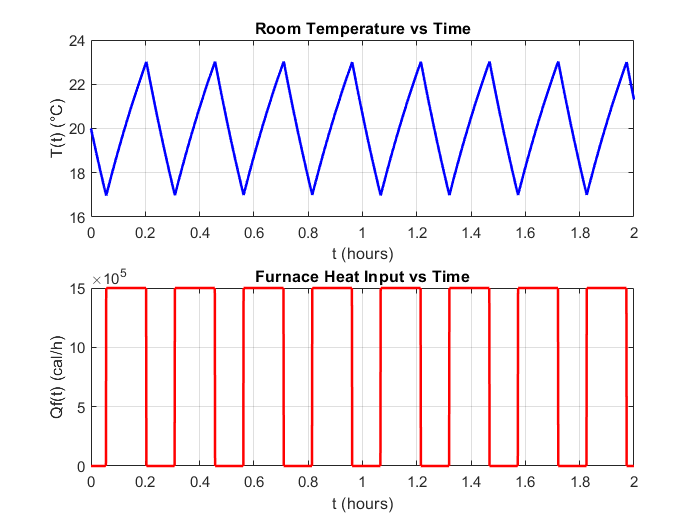
\includegraphics[width=\textwidth]{Figures/figure22.png}
    \caption{Temperature and Furnace Input Over Time}
    \label{fig:figure22} 
  \end{figure}

  % ANSWER TO 2.3
  \item 
  To calculate the number of standard cubic meters of natural gas consumed, we follow the below equation:

  Define $t_{on} \triangleq$  time the furnace was on in hours. The Matlab code says it was 1.182 hours\\
  Define $Q_{f,on} \triangleq$ as the furnace heat input. \\
  Define $\rho_e \triangleq$ as the energy density. \\
  Define $e \triangleq$ as the efficiency. \\

  \[
  \text{Volume of gas consumed} = \frac{t_{on} Q_{f,\text{on}}}{\rho_e e} = \frac{(1.182)(1.5 \times 10^6)}{(9 \times 10^6)(0.9)} = 0.2188888
  \]
  \[
  \approx 0.219 \, \text{standard cubic meters}
  \]

  We also confirm with unit analysis that we get cubic meters.

  \[
  \text{Volume of gas consumed} = \frac{t_{\text{on}} Q_{f,\text{on}}}{\rho_e e} = \frac{\text{hour} \cdot \frac{\text{cal}}{\text{hour}}}{\frac{\text{cal}}{\text{m}^3}} = \text{m}^3
  \]

  % ANSWER TO 2.4
  \item
  With a new oscillating defintion of Ta, we get Figure 2 below demonstrating the temperature and furnace input over time.

  \begin{figure}[h!]
    \centering
    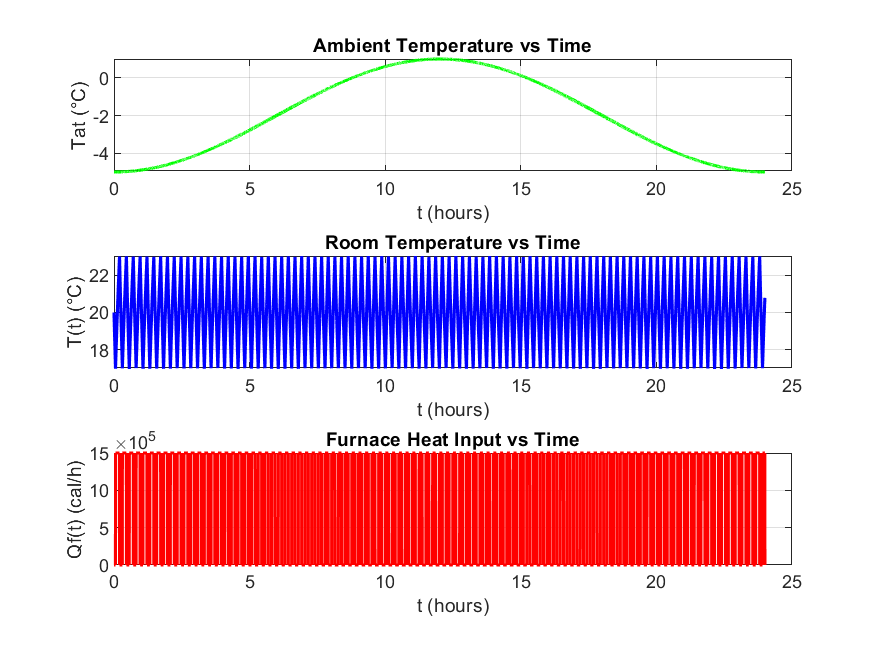
\includegraphics[width=\textwidth]{Figures/figure24.png}
    \caption{Temperature and Furnace Input Over Time}
    \label{fig:figure24}
  \end{figure}

  The simulation results align with the expected behavior of the system. The room temperature \( T(t) \) is maintained within the desired range of \( 17^\circ \text{C} \) to \( 23^\circ \text{C} \) as the furnace responds to changes in the ambient temperature \( T_a(t) \). When \( T_a(t) \) is lower, the furnace operates more frequently to offset increased heat loss, while at higher \( T_a(t) \), the furnace operates less often due to reduced heat loss. This behavior reflects the thermal dynamics of the system and the influence of the bang-bang control logic.


  \end{enumerate}
\newpage

\item Question 3
  \begin{enumerate}
  \item Part A  % This will appear as "3.1"

  SOLUTION

  \item Part B  % This will appear as "3.2"

  SOLUTION
  \end{enumerate}
\newpage

\item Question 4
  \begin{enumerate}
  \item Part A  % This will appear as "4.1"

  SOLUTION

  \item Part B  % This will appear as "4.2"

  SOLUTION
  \end{enumerate}
\newpage

\item Question 5
  \begin{enumerate}
  \item Part A  % This will appear as "5.1"

  SOLUTION

  \item Part B  % This will appear as "5.2"

  SOLUTION
  \end{enumerate}
\newpage

\end{enumerate}
\end{document}
